\documentclass[12pt, a4paper]{article}
\usepackage[utf8]{inputenc}
\usepackage[T1]{fontenc}
\usepackage[norsk]{babel}
\usepackage{hyperref}
\usepackage{fancyvrb}


\usepackage{tikz}
\usepackage{circuitikz}
\usepackage{amsmath}

\usetikzlibrary{automata}
\usetikzlibrary{shapes}
\usetikzlibrary{circuits}

\title{Tegnekurs i TikZ}
\author{Veronika Heimsbakk \\ veronahe@ulrik.uio.no}

\begin{document}

\maketitle
\tableofcontents
\newpage

%%% BASICS %%%
\section{The Basics}
For å kunne bruke pakken TikZ må man først inkludere \texttt{\textbackslash usepackage\{tikz\}} i dokumentet sitt. 

\subsection{\texttt{tikzpicture}}
Alle illustrasjoner som skal tegnes ved hjelp av pakken TikZ krever et miljø som heter \texttt{tikzpicture}.

\begin{Verbatim}[fontsize=\small]
\begin{tikzpicture}
    <kode her>
\end{tikzpicture}
\end{Verbatim}

\subsection{Linjer}

\begin{center}
\begin{tikzpicture}
	\draw (0,2) -- (4,2);
	\draw (0cm,1.5cm) -- (4cm,1.5cm);
	\draw (0em, 1cm) -- (4em, 1cm);
	\draw (0pt, 0.5cm) -- (4pt, 0.5cm);
\end{tikzpicture}
\end{center}

En av de mest brukte TikZ kommandoene er \texttt{\textbackslash draw}. For å tegne ei rett linje sier man hvor man vil tegne \textit{fra} og \textit{til}:

\begin{Verbatim}[fontsize=\small, frame=single]
\draw (0,2) -- (4,2);
\draw (0cm,1.5cm) -- (4cm,1.5cm);
\draw (0em, 1cm) -- (4em, 1cm);
\draw (0pt, 0.5cm) -- (4pt, 0.5cm);
\end{Verbatim}

\subsection{Kurver}
Vi bruker kontrollpunkter for å lage en kurvet linje. I eksempelet her, så starter vi i koordinatene \texttt{(-2,2)} og så tegner vi en kurve til første kontrollpunkt som er \texttt{(-1,0)}, så videre til \texttt{(1,0)}, og til slutt ender kurven opp i slutt-punktet som er \texttt{(2,2)}.

\begin{center}
\begin{tikzpicture}
	\draw (-2,2) .. controls (-1,0) and (1,0) .. (2,2);
\end{tikzpicture}
\end{center}

\begin{Verbatim}[fontsize=\small]
\draw (-2,2) .. controls (-1,0) and (1,0) .. (2,2);
\end{Verbatim}

\newpage

\subsection{Kvadrat}
\noindent Videre kan vi bygge på og lage et kvadrat:
\begin{center}
\begin{tikzpicture}
	\draw (0,0) rectangle (2,2);
\end{tikzpicture}
\end{center}

\begin{Verbatim}[fontsize=\small]
\draw (0,0) -- (2,0) -- (2,2) -- (0,2) -- (0,0);
\end{Verbatim}

Vi kan også bruke nøkkelordet \texttt{rectangle}, og lage en kortversjon som gjør akkurat det samme:
\begin{Verbatim}[fontsize=\small]
\draw (0,0) rectangle (2,2);
\end{Verbatim}

\subsection{Sirkel}
\begin{center}
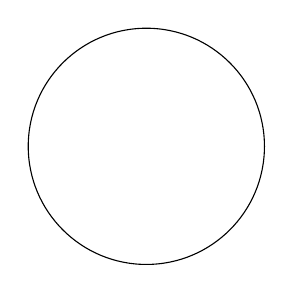
\begin{tikzpicture}
	\draw (2,2) circle (1.5cm);
\end{tikzpicture}
\end{center}

Den første koordinaten er sirkelens sentrum, og lengden vi oppgir til slutt er sirkelens radius.
\begin{Verbatim}[fontsize=\small]
\draw (2,2) circle (1.5cm);
\end{Verbatim}

\noindent Ellipser tegnes ved at vi oppgir radiusen i x- og y-retningene:
\begin{center}
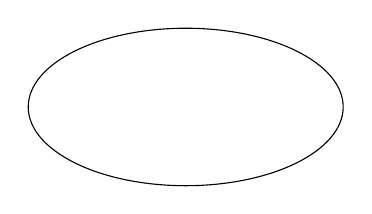
\begin{tikzpicture}
	\draw (2,2) ellipse (2cm and 1cm);
\end{tikzpicture}
\end{center}

\begin{Verbatim}[fontsize=\small]
\draw (2,2) ellipse (2cm and 1cm);
\end{Verbatim}

\subsection{Pynte litt}
For å pynte litt på sirkelen vår, kan vi legge til noen ekstra argumenter til \texttt{\textbackslash draw}-kommandoen. For eksempel slik:
\begin{center}

\begin{tikzpicture}
	\draw[red, thick, dashed] (2,2) circle (1cm);
	\draw[green, thick] (6,2) circle (1cm);
\end{tikzpicture}
\end{center}

\begin{Verbatim}[fontsize=\small]
\draw[red, thick, dashed] (2,2) circle (1cm);
\draw[green, thick] (6,2) circle (1cm);
\end{Verbatim}


\subsection{Tykkelser}
\begin{figure}[h!]
\centering
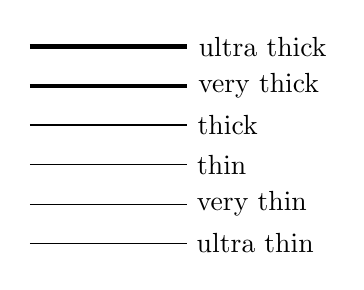
\begin{tikzpicture}
	\draw[ultra thin] (0,0) -- (2,0) node[right] {ultra thin};
	\draw[very thin] (0,0.5) -- (2,0.5) node[right] {very thin};
	\draw[thin] (0,1) -- (2,1) node[right] {thin};
	\draw[thick] (0,1.5) -- (2,1.5) node[right] {thick};
	\draw[very thick] (0,2) -- (2,2) node[right] {very thick};'
	\draw[ultra thick] (0,2.5) -- (2,2.5) node[right] {ultra thick};
\end{tikzpicture}
\caption{Mulige tykkelser i TikZ.}
\end{figure}


\subsection{Farger}
\begin{figure}[h!]
\centering
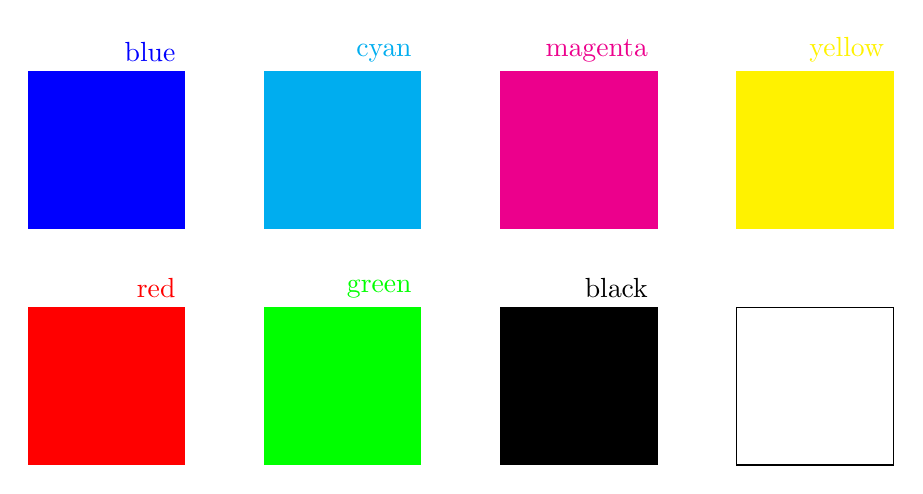
\begin{tikzpicture}
	\fill[red] (0,0) rectangle (2,2) node[above left] {red};
	\fill[green] (3,0) rectangle (5,2) node[above left] {green};
	\fill[black] (6,0) rectangle (8,2) node[above left] {black};
	\filldraw[white, draw=black, thin] (9,0) rectangle (11,2) node[above left] {white};
	\fill[blue] (0,3) rectangle (2,5) node[above left] {blue};
	\fill[cyan] (3,3) rectangle (5,5) node[above left] {cyan};
	\fill[magenta] (6,3) rectangle (8,5) node[above left] {magenta};
	\fill[yellow] (9,3) rectangle (11,5) node[above left] {yellow};
\end{tikzpicture}
\caption{Mulige farger i TikZ.}
\end{figure}


\subsection{Bruke farger}
Vi kan også fylle formene våre ved å bruke kommandoen \texttt{\textbackslash fill}.

\begin{center}

\begin{tikzpicture}
	\fill[red] (0,0) rectangle (2,2);
\end{tikzpicture}
\end{center}

\begin{Verbatim}[fontsize=\small]
\fill[red] (0,0) rectangle (2,2);
\end{Verbatim}

\noindent Om vi ønsker å legge til en kant rundt kvadratet, kan vi bruke kommandoen \texttt{\textbackslash filldraw}. Her fyller vi kvadratet rødt med gjennomsiktighet på 50\% og en tykk sort strek som kant.

\begin{center}
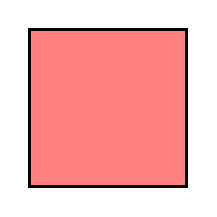
\begin{tikzpicture}
	\filldraw[red!50, draw=black, very thick] (0,0) rectangle (2,2);
\end{tikzpicture}
\end{center}

\begin{Verbatim}[fontsize=\small]
\filldraw[red!50, draw=black, very thick] (0,0) rectangle (2,2);
\end{Verbatim}

\noindent Vi har også gradient i TikZ, og det kan se slik ut:

\vspace{15pt}

\begin{center}
\begin{minipage}{0.3\textwidth}

\begin{tikzpicture}
	\shade[left color=black, right color=red] (0,0) rectangle (2,2);
\end{tikzpicture}
\end{minipage}
\begin{minipage}{0.3\textwidth}

\begin{tikzpicture}
	\shade[top color=black, bottom color=red] (0,0) rectangle (2,2);
\end{tikzpicture}
\end{minipage}
\begin{minipage}{0.3\textwidth}

\begin{tikzpicture}
	\shade[inner color=black, outer color=red] (0,0) rectangle (2,2);
\end{tikzpicture}
\end{minipage}
\end{center}
\vspace{10pt}


\begin{Verbatim}[fontsize=\small]
\shade[left color=black, right color=red]  (0,0) rectangle (2,2);
\shade[top color=black, bottom color=red]  (0,0) rectangle (2,2);
\shade[inner color=black, outer color=red] (0,0) rectangle (2,2);
\end{Verbatim}

\newpage

%%% KOORDINATER %%%
\section{Koordinatsystem}
Dette eksempelet krever et rutenett, piler, noder og plassering av tall og bokstaver. Vi starter med et rutenett:

\begin{center}
\scalebox{0.8}{
\begin{tikzpicture}
    \draw[step=1cm,gray!80,very thin] (-1.9,-1.9) grid (5.9,5.9);
\end{tikzpicture}
}
\end{center}

\begin{Verbatim}[fontsize=\small]
\draw[step=1cm,gray!80,very thin] (-1.9,-1.9) grid (5.9,5.9);
\end{Verbatim}


\subsection{Piler/akser}
\noindent Videre trenger vi x-aksen og y-aksen. Dette er to linjer med piler i enden.

\begin{center}
\scalebox{0.8}{
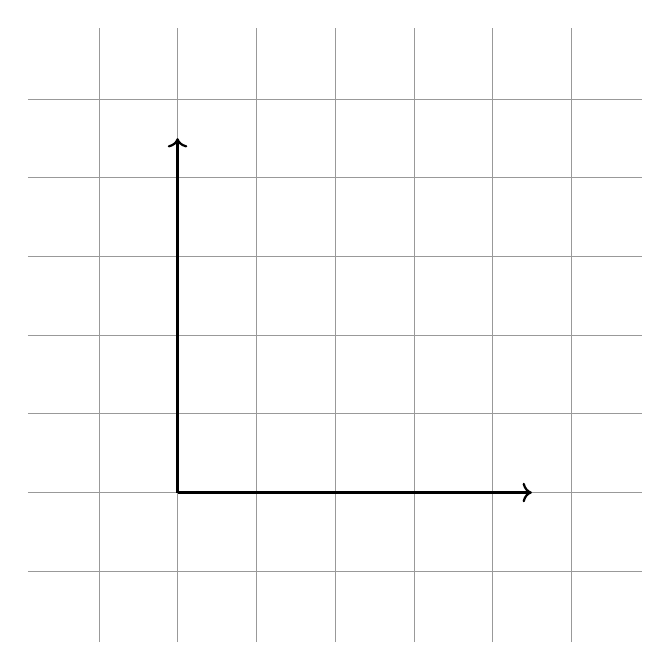
\begin{tikzpicture}
    \draw[step=1cm,gray!80,very thin] (-1.9,-1.9) grid (5.9,5.9);
    \draw[thick, ->] (0,0) -- (4.5,0);
    \draw[thick, ->] (0,0) -- (0,4.5);
\end{tikzpicture}
}
\end{center}

\begin{Verbatim}[fontsize=\small]
\draw[thick, ->] (0,0) -- (4.5,0);
\draw[thick, ->] (0,0) -- (0,4.5);
\end{Verbatim}

\newpage
\subsection{Noder}
Vi kan legge på tekst (\textit{label}) ved å bruke nøkkelordet \texttt{node}. Vi plasserer teksten ved linjene vi har tegnet ved å fortelle noden hvor vi vil ha den.

\begin{center}
\scalebox{0.6}{
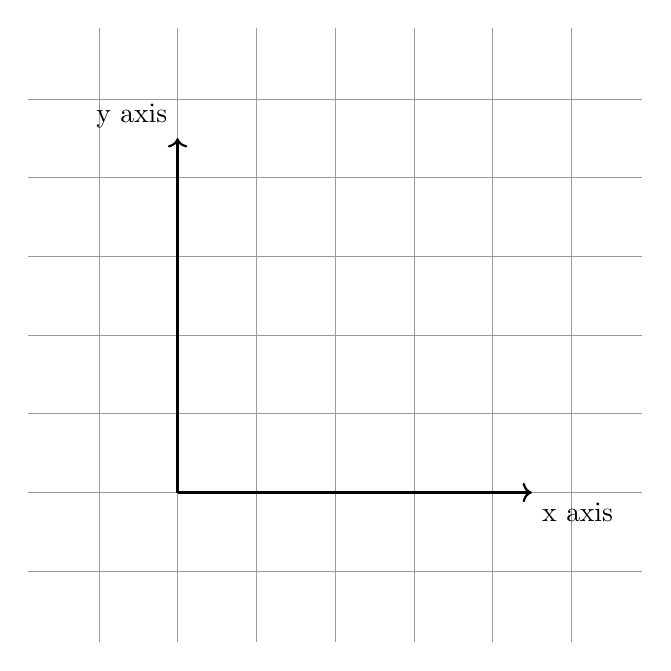
\begin{tikzpicture}
    \draw[step=1cm,gray!80,very thin] (-1.9,-1.9) grid (5.9,5.9);
    \draw[thick, ->] (0,0) -- (4.5,0) node[below right] {x axis};
    \draw[thick, ->] (0,0) -- (0,4.5) node[above left] {y axis};
\end{tikzpicture}
}
\end{center}

\begin{Verbatim}[fontsize=\small]
\draw[thick, ->] (0,0) -- (4.5,0) node[below right] {x axis};
\draw[thick, ->] (0,0) -- (0,4.5) node[above left] {y axis};
\end{Verbatim}


\subsection{Løkker}
\noindent Vi kan fortsette med tallene som skal gå langs aksene ved å bruke løkker:
\begin{center}
\scalebox{0.6}{
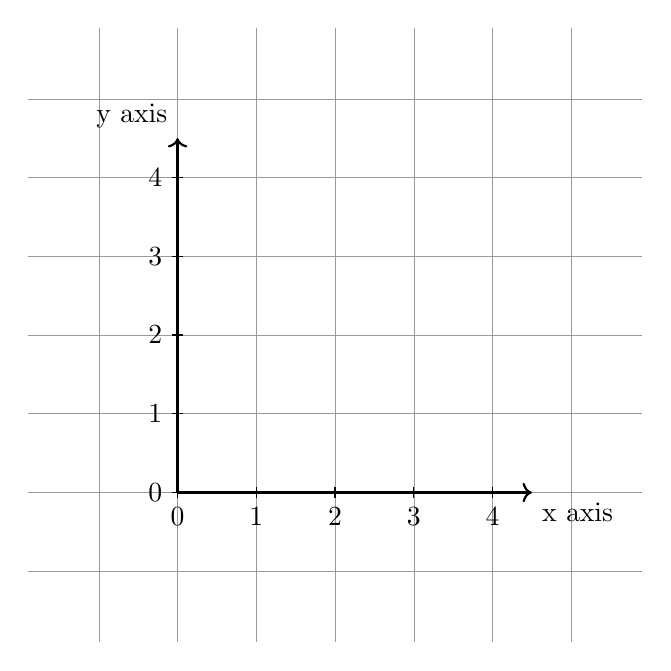
\begin{tikzpicture}
    \draw[step=1cm,gray!80,very thin] (-1.9,-1.9) grid (5.9,5.9);
    \draw[thick, ->] (0,0) -- (4.5,0) node[below right] {x axis};
    \draw[thick, ->] (0,0) -- (0,4.5) node[above left] {y axis};

    \foreach \x in {0,1,2,3,4}
	\draw (\x cm, 2pt) -- (\x cm, -2pt) node[below] {$\x$};
    \foreach \y in {0,1,2,3,4}
	\draw (2pt, \y cm) -- (-2pt, \y cm) node[left] {$\y$};
\end{tikzpicture}
}
\end{center}

Denne løkken går over linjene vi allerede har tegnet, og setter en liten strek for hver centimeter. Og ved siden av linjen skriver vi et tall.

\begin{Verbatim}[fontsize=\small, frame=single]
\foreach \x in {0,1,2,3,4}
  \draw (\x cm, 2pt) -- (\x cm, -2pt) node[below] {$\x$};
\foreach \y in {0,1,2,3,4}
  \draw (2pt, \y cm) -- (-2pt, \y cm) node[left]  {$\y$};
\end{Verbatim}

\subsection{Hele koden for koordinatsystemet}
\begin{center}
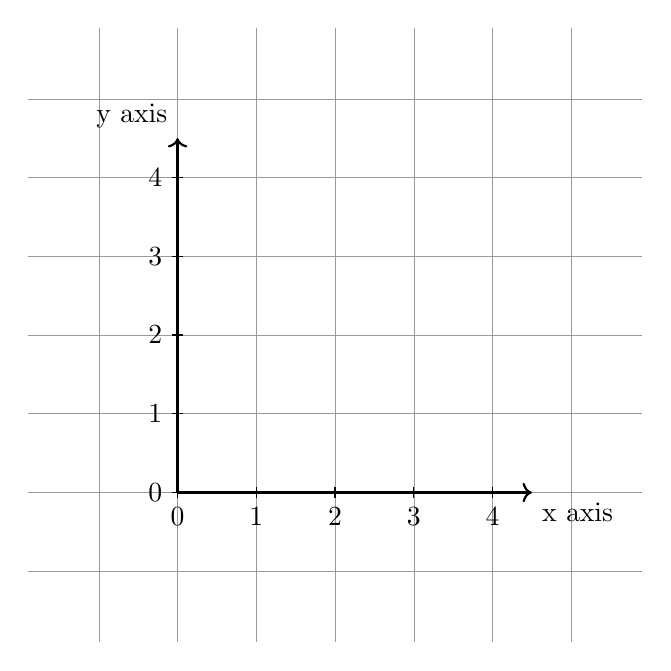
\begin{tikzpicture}
    \draw[step=1cm,gray!80,very thin] (-1.9,-1.9) grid (5.9,5.9);
    \draw[thick, ->] (0,0) -- (4.5,0) node[below right] {x axis};
    \draw[thick, ->] (0,0) -- (0,4.5) node[above left] {y axis};

    \foreach \x in {0,1,2,3,4}
	\draw (\x cm, 2pt) -- (\x cm, -2pt) node[below] {$\x$};
    \foreach \y in {0,1,2,3,4}
	\draw (2pt, \y cm) -- (-2pt, \y cm) node[left] {$\y$};
\end{tikzpicture}
\end{center}

\begin{Verbatim}[fontsize=\small, frame=single]
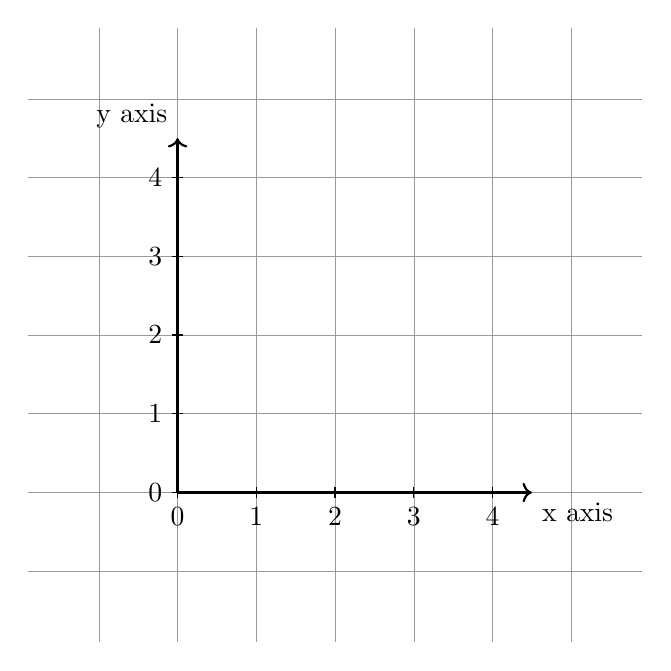
\begin{tikzpicture}
  \draw[step=1cm,gray!80,very thin] (-1.9,-1.9) grid (5.9,5.9);
  \draw[thick, ->] (0,0) -- (4.5,0) node[below right] {x axis};
  \draw[thick, ->] (0,0) -- (0,4.5) node[above left] {y axis};

  \foreach \x in {0,1,2,3,4}
    \draw (\x cm, 2pt) -- (\x cm, -2pt) node[below] {$\x$};
  \foreach \y in {0,1,2,3,4}
    \draw (2pt, \y cm) -- (-2pt, \y cm) node[left] {$\y$};
\end{tikzpicture}
\end{Verbatim}

\newpage

%%% TRÆR %%%
\section{Trær}
Et tre består av en rekke noder. Når vi tegner trær i TikZ starter vi med å definere rot-noden. Legg merke til attributtene vi git \texttt{tikzpicture}. Her sier vi at \texttt{every node} skal ha \textit{stilen} (\texttt{.style}) sirkel med sort strek.

\begin{center}

\begin{tikzpicture}[every node/.style={circle, draw=black},level 2/.style={sibling distance=20mm},
				   level 3/.style={sibling distance=10mm}, level distance=30pt]
\node {1};
\end{tikzpicture}
\end{center}

\begin{Verbatim}[fontsize=\small, frame=single]

\begin{tikzpicture}[every node/.style={circle, draw=black}]
    \node {1};
\end{tikzpicture}
\end{Verbatim}

\subsection{Bygge treet}
Treet bygger vi ved å legge til barna. Barna skrives på formen:
\begin{Verbatim}[fontsize=\small]
child { node[opt.] {value} }
\end{Verbatim}

\begin{center}
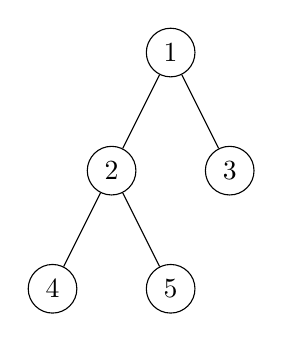
\begin{tikzpicture}[every node/.style={circle, draw=black}]
\node {1}
	child { node {2} 
		child { node {4} }
		child { node {5} }
	}
	child { node {3} }
;
\end{tikzpicture}
\end{center}

\begin{Verbatim}[fontsize=\small, frame=single]
\node {1}
    child { node {2} 
        child { node {4} }
        child { node {5} }
    }
    child { node {3} }
;
\end{Verbatim}

\newpage

\subsection{Justere avstand mellom noder}

Når vi nå vil bygge videre og legge til tallet 6 under \texttt{child \{node \{3\}\}} vil vi krasje bort i 5. Da trenger vi å justere avstanden mellom søsken-noder.

\vspace{20pt}

\begin{minipage}{0.5\textwidth}
Vi har: \newline \newline
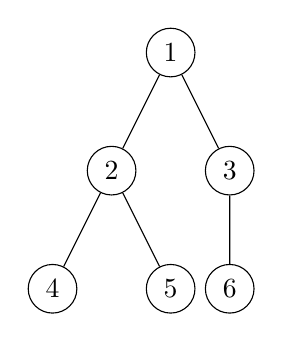
\begin{tikzpicture}[every node/.style={circle, draw=black}]
\node {1}
	child { node {2} 
		child { node {4} }
		child { node {5} }
	}
	child { node {3} 
		child { node {6} }
	}
;
\end{tikzpicture}
\end{minipage}
\begin{minipage}{0.5\textwidth}
Vi vil ha: \newline \newline
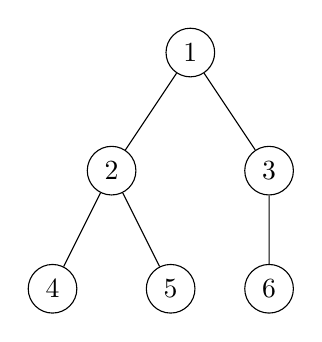
\begin{tikzpicture}[every node/.style={circle, draw=black}, 
				   level 1/.style={sibling distance=20mm}, 
				   level 2/.style={sibling distance=15mm}]
\node {1}
	child { node {2} 
		child { node {4} }
		child { node {5} }
	}
	child { node {3} 
		child {node {6} }
	}
;
\end{tikzpicture}
\end{minipage}

\vspace{20pt}

Da legger vi på at attributt til i listen til \texttt{tikzpicture} som forteller noe om avstanden mellom nodene. 

\begin{Verbatim}[fontsize=\small, frame=single]
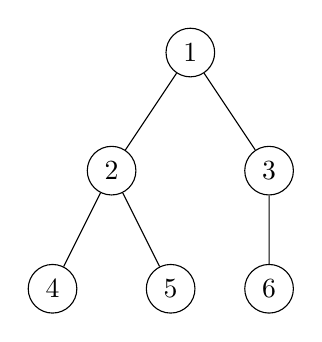
\begin{tikzpicture}[every node/.style={circle, draw=black}, 
		    level 1/.style={sibling distance=20mm}, 
		    level 2/.style={sibling distance=15mm}]

\node {1}
    child { node {2} 
        child { node {4} }
        child { node {5} }
    }
    child { node {3} 
        child {node {6} }
    }
;
\end{tikzpicture}
\end{Verbatim}

Her forteller vi at stilen til nodene på \texttt{level 1} skal være at de har avstand til sine søsken med 20 mm, og 15 mm for \texttt{level 2}. Vi kunne også lagt til attributtet \texttt{level distance} for å få større eller mindre avstand mellom lagene. 

\newpage

\subsection{Former som noder kan ha}
Man kan få forskjellige fasonger på noder ved å inkludere \texttt{\textbackslash usetikzlibrary\{shapes\}}. Her er en oversikt over forskjellige fasonger en node kan ha. For å få ønsket fasong skriver man noden på denne formen:
\begin{Verbatim}[fontsize=\small, frame=single]
\node[rectangle] {Rectangle};
\node[regular polygon, regular polygon sides=5] {n=5};
\node[star, star points=4] {p=4};
\node[circle split] {Circle \nodepart{lower} split};
\end{Verbatim}

\begin{figure}[h!]
\centering
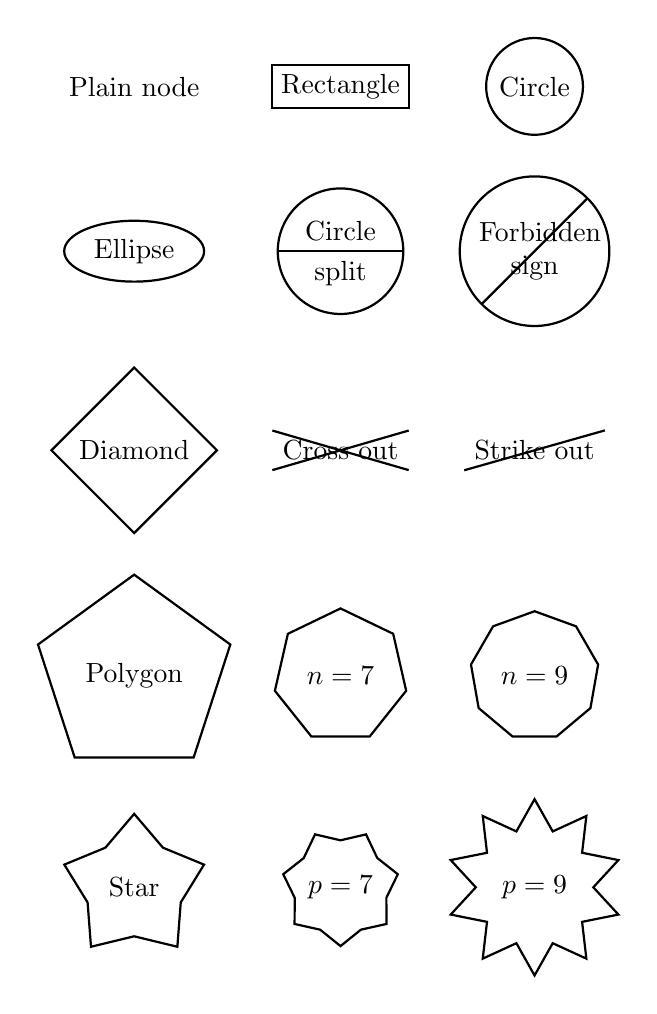
\begin{tikzpicture}
    \matrix[nodes={draw, thick},
        row sep=0.5cm,column sep=0.5cm] {
    \node[draw=none,fill=none] {Plain node}; &
    \node[rectangle] {Rectangle}; &
    \node[circle] {Circle};\\
    \node[ellipse] {Ellipse};&
    \node[circle split] {Circle \nodepart{lower} split};&
    \node[forbidden sign,text width=4em, text centered] {Forbidden sign};\\
    \node[diamond] {Diamond};&
    \node[cross out] {Cross out};&
    \node[strike out] {Strike out};\\
    \node[regular polygon,regular polygon sides=5] {Polygon};&
    \node[regular polygon,regular polygon sides=7] {$n=7$};&
    \node[regular polygon,regular polygon sides=9] {$n=9$};\\
    \node[star] {Star};&
    \node[star,star points=7,star point ratio=0.8] {$p=7$};&
    \node[star,star points=10] {$p=9$};\\
    };
\end{tikzpicture}
\caption{Forskjellige fasonger på noder.}
\end{figure}


\newpage

\subsection{Eksempel på et tre med avstander}

\begin{center}
\begin{tikzpicture}[every node/.style={},level 2/.style={sibling distance=20mm},
				   level 3/.style={sibling distance=10mm}, level distance=30pt]
\node {S}
	child { node{A} 
		child { node {A} 
			child { node {(} }
			child { node {)} }
		}
		child { node {A} 
			child { node {(} }
			child { node {A} 
				child { node {(} }
				child { node {)} }
			}
			child { node {)} }
		}
	};
\end{tikzpicture}
\end{center}

\begin{Verbatim}[fontsize=\small, frame=single]
\begin{tikzpicture}[every node/.style={},
                    level 2/.style={sibling distance=20mm},
                    level 3/.style={sibling distance=10mm}, 
                    level distance=30pt]
\node {S}
    child { node{A} 
        child { node {A} 
            child { node {(} }
            child { node {)} }
        }
        child { node {A} 
            child { node {(} }
            child { node {A} 
                child { node {(} }
                child { node {)} }
            }
            child { node {)} }
        }
    }
;
\end{tikzpicture}
\end{Verbatim}

\newpage

\subsection{Rød-svarte trær}

\tikzset{
	treenode/.style = {align=center, inner sep=0pt},
	% Sorte noder
  	node_black/.style = {treenode, circle, white, font=\bfseries, draw=black,fill=black, text width=0.8cm},
	% Røde noder
  	node_red/.style = {treenode, circle, red, draw=red, text width=0.8cm, very thick},
	% Null-pekere
  	node_null/.style = {treenode, rectangle, draw=black, minimum width=0.3cm, minimum height=0.3cm}
}
\begin{center}
% Skal tegne med piler (->), og setter level/.style={opt.} %
\begin{tikzpicture}[->,level/.style={sibling distance = 2cm, level distance = 1.5cm}] 
\node [node_black] {38}
    	child{ node [node_red] {19} 
		child{node [node_black] {12}
			child{node [node_red] {8}}
			child{node [node_null] {}}
		}
		child{node [node_black] {31}}
	}
    	child{ node [node_black] {41} }
; 
\end{tikzpicture}
\end{center}

Å tegne trær på denne måten krever ingen tilleggsbiblioteker fra TikZ. Dette er et eksempel på tegning med \textit{parametre}. Utseende til nodene i treet er definert som parametre som har et sett med \texttt{.style}-opsjoner.
\begin{Verbatim}[fontsize=\small, frame=single]
\tikzset{
   treenode/.style = {align=center, inner sep=0pt},
	
   % Sorte noder
   node_black/.style = {treenode, circle, white, 
			font=\bfseries, draw=black,
			fill=black, text width=0.8cm},
   % Røde noder
   node_red/.style = {treenode, circle, red, draw=red, 
	              text width=0.8cm, very thick},
   % Null-pekere
   node_null/.style = {treenode, rectangle, draw=black, 
		       minimum width=0.3cm, minimum height=0.3cm}
}
\end{Verbatim}
Starter med å definere \texttt{treenode}, som er felles for alle typer noder. Røde og sorte noder tegnes som \texttt{circle}, hvor sorte noder har \texttt{fill=black} og tekstfarge \texttt{white}, mens røde noder har rødt omriss med \texttt{draw=red}, og tekstfarge \texttt{red}. Null-nodene sier vi skal være sorte \texttt{rectangle}. Tegnes som små kvadrater på 0.3 cm $\times$ 0.3 cm.

\newpage
\subsection{Bygge et tre}
\begin{Verbatim}[fontsize=\small, frame=single]
\begin{tikzpicture}[->,level/.style={ sibling distance = 2cm, 
                    level distance = 1.5cm }] 
\node [node_black] {38}
    child {node [node_red] {19} 
        child {node [node_black] {12}
             child {node [node_red] {8} }
             child {node [node_null] {} }
        }
        child {node [node_black] {31} }
    }
    child { node [node_black] {41} }
; 
\end{tikzpicture}
\end{Verbatim}

Setter forskjellige opsjoner med:
\begin{center}
\texttt{\{tikzpicture\}[->, level/.style=\{sibling distance=2cm, level distance)=1.5cm\}]}
\end{center}
Her sier vi at treet skal tegnes med piler (\texttt{->}), og at stilen (\texttt{.style}) for distansen mellom søskennoder skal være 2 cm, og distansen mellom barn og foreldre skal være 1.5 cm.

Videre så tegnes treet ved å definere roten:
\begin{center}
\texttt{\textbackslash node [opt.] \{node value\} ;} 
\end{center}
Så kan man bygge treet ved å legge inn barna til roten, osv.:
\vspace{1em}

\texttt{\textbackslash node [opt.] \{node value\} \\
\indent \indent child \{node [opt.] \{node value\} \} ;} 

\newpage

%%% GRAFER %%%
\section{Grafer}

\begin{center}
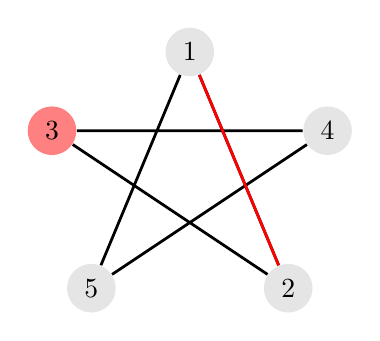
\begin{tikzpicture}[scale=5]
	 \tikzstyle{vertex}=[circle,fill=black!10]
	 \tikzstyle{selected vertex} = [vertex, fill=red!50]

	 \tikzstyle{selected edge} = [draw,line width=1pt,-,red!100]
	 \tikzstyle{edge} = [-,black,line width=1pt]

	 \node[vertex] (v1) at (1.25,1.7) 			{1};
	 \node[vertex] (v2) at (1.5,1.1) 				{2};
	 \node[selected vertex] (v3) at (0.9,1.5) 		{3};
	 \node[vertex] (v4) at (1.6,1.5) 				{4};
	 \node[vertex] (v5) at (1,1.1) 				{5};

	\draw[edge] (v1)  -- (v2) -- (v3) -- (v4) -- (v5) -- (v1); 
	\draw[selected edge] (v1) -- (v2);
\end{tikzpicture}
\end{center}

Det fins enklere måter å tegne grafer på enn dette, men jeg syns denne måten er fin. Den krever heller ingen andre biblioteker eller pakker enn TikZ selv. Eksempel på en veldig mye enklere måte kommer på slutten av denne seksjonen.

Vi starter med å definere de forskjellige elementene til en graf.

\begin{Verbatim}[fontsize=\small, frame=single]
\begin{tikzpicture}
    \tikzstyle{vertex} = [circle,fill=black!10]
    \tikzstyle{selected vertex} = [vertex, fill=red!50]

    \tikzstyle{selected edge} = [draw,line width=1pt,-,red!100]
    \tikzstyle{edge} = [-,black,line width=1pt]
\end{tikzpicture}
\end{Verbatim}
Her fortelle vi at \texttt{vertex}er (eller noder), skal være sirkler som er fylt med sort med en gjennomsiktighet på 10\%. Markerte noder skal også være fylt, da med en annen farge.
\begin{center}

\begin{tikzpicture}[scale=2]
	 \tikzstyle{vertex}=[circle,fill=black!10]
	 \tikzstyle{selected vertex} = [vertex, fill=red!50]

	 \node[vertex] (v1) at (1,1) 				{x};
	 \node[selected vertex] (v2) at (2,1) 		{y};
\end{tikzpicture}
\end{center}

\noindent Kanter skal tegnes som sorte linjer (\texttt{[-, black $\dots$]}). Og markerte kanter skal være røde.

\begin{center}
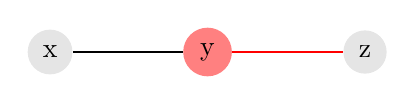
\begin{tikzpicture}[scale=2]
	 \tikzstyle{vertex}=[circle,fill=black!10]
	 \tikzstyle{selected vertex} = [vertex, fill=red!50]
	 \tikzstyle{selected edge} = [draw,line width=1pt,-,red!100]
	 \tikzstyle{edge} = [-,black,line width=1pt]

	 \node[vertex] (v1) at (1,1) 				{x};
	 \node[selected vertex] (v2) at (2,1) 		{y};
	\node[vertex] (v3) at (3,1)					{z};
	\draw[edge] (v1) -- (v2);
	\draw[selected edge] (v2) -- (v3);
\end{tikzpicture}
\end{center}

\newpage
\subsection{Tegne grafen} For å plassere nodene rundt om på arket sier man hvor man vil de skal være. For eksempelet på toppen (grafen som har stjerne-form), er TikZ-koden som følger:

\begin{Verbatim}[fontsize=\small, frame=single]
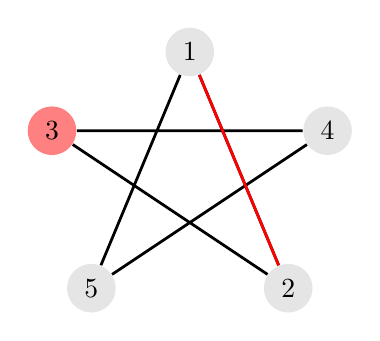
\begin{tikzpicture}[scale=5]
    \tikzstyle{vertex}          = [circle,fill=black!10]
    \tikzstyle{selected vertex} = [vertex, fill=red!50]

    \tikzstyle{selected edge}   = [draw,line width=1pt,-,red!100]
    \tikzstyle{edge}            = [-,black,line width=1pt]

    \node[vertex]          (v1) at (1.25,1.7) {1};
    \node[vertex]          (v2) at (1.5,1.1)  {2};
    \node[selected vertex] (v3) at (0.9,1.5)  {3};
    \node[vertex]          (v4) at (1.6,1.5)  {4};
    \node[vertex]          (v5) at (1,1.1)    {5};

    \draw[edge]          (v1)--(v2)--(v3)--(v4)--(v5)--(v1); 
    \draw[selected edge] (v1)--(v2);
\end{tikzpicture}
\end{Verbatim}

\newpage

%%% AUTOMATER %%%
\section{Automater}

\begin{center}

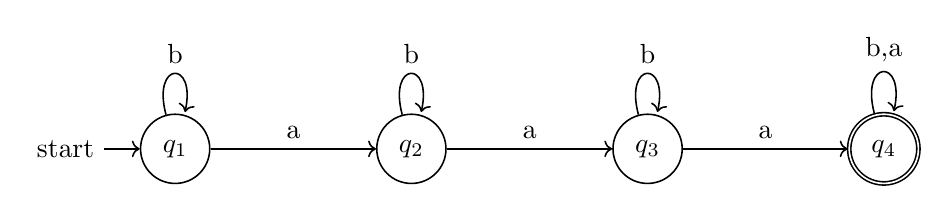
\begin{tikzpicture}[->,auto,node distance=3cm,line width=0.2mm]
  \node[initial,state] 			(A)		 	         {$q_1$};
  \node[state]         			(B) [right of=A] 	{$q_2$};
  \node[state]				(C) [right of=B] 	{$q_3$};
  \node[state,accepting]		(D) [right of=C] 	{$q_4$};

  \path 	(A) edge [loop above] node 			{b} 		(A)
			edge node 						{a} 		(B)
        		(B) edge [loop above] node 			{b} 		(B)
			edge node 						{a} 		(C)
		(C) edge [loop above] node 			{b}		(C)
			edge node 						{a} 		(D)
		(D) edge [loop above] node 			{b,a}	(D);
\end{tikzpicture}
\end{center}

\begin{Verbatim}[fontsize=\small, frame=single]
\begin{tikzpicture}[->,auto,node distance=3cm,line width=0.2mm]
  \node[initial,state   (A) 		{$q_1$};
  \node[state]          (B) [right of=A]    {$q_2$};
  \node[state]	  (C) [right of=B]    {$q_3$};
  \node[state,accepting](D) [right of=C]    {$q_4$};

  \path (A) edge [loop above] node 	 {b}   (A)
	    edge node      		 {a}   (B)
        (B) edge [loop above] node 	 {b}   (B)
	    edge node   	  	  {a}   (C)
        (C) edge [loop above] node	  {b}   (C)
	    edge node 	    	  {a}   (D)
        (D) edge [loop above] node 	 {b,a} (D);
\end{tikzpicture}
\end{Verbatim}


For denne måten å tegne automater på, så settes alle parametre som beskriver automaten i definisjonen til \texttt{tikzpicture}. Man må også inkludere \texttt{\textbackslash usetikzlibrary\{automata\}}.
Her har automaten følgende egenskaper:
\begin{center}
\texttt{\{tikzpicture\}[->, auto, node distance=3cm, line width=0.2mm]}
\end{center}
Dette forteller oss at automaten skal tegnes med piler (\texttt{->}), nodene skal ha avstand på 3 cm, og linjene en tykkelse på 0,2 mm. Auto stiller teksten \textit{over} linjene, i stedet for \textit{på} linjene.

\subsection{Automatens tilstander} En automat har tre typer tilstander: starttilstanden, vanlig tilstand(er), og akepterende tilstand(er).
\begin{center}
\texttt{\textbackslash node[state] (node-name) \{name of state\};}
\end{center}
I tillegg til \texttt{[state]}, så kan man ha med opsjonen \texttt{[initial, state]} for starttilstanden, eller \texttt{[state, accepting]} for aksepterende tilstand.

\subsection{Stien gjennom automaten}
Stien tegnes gjennom en \texttt{path}. Denne konstrueres på følgende vis:
\begin{center}
\texttt{\textbackslash path (from-node) edge [opt.] node \{weight\} (to-node)}.
\end{center}
Her kan \texttt{[opt]} være \texttt{loop above/below}, \texttt{bend left/right}.

\subsection*{Flittig bever}
Her er en flittig 4-bever. Denne automaten dekker de fleste opsjoner.
\begin{center}
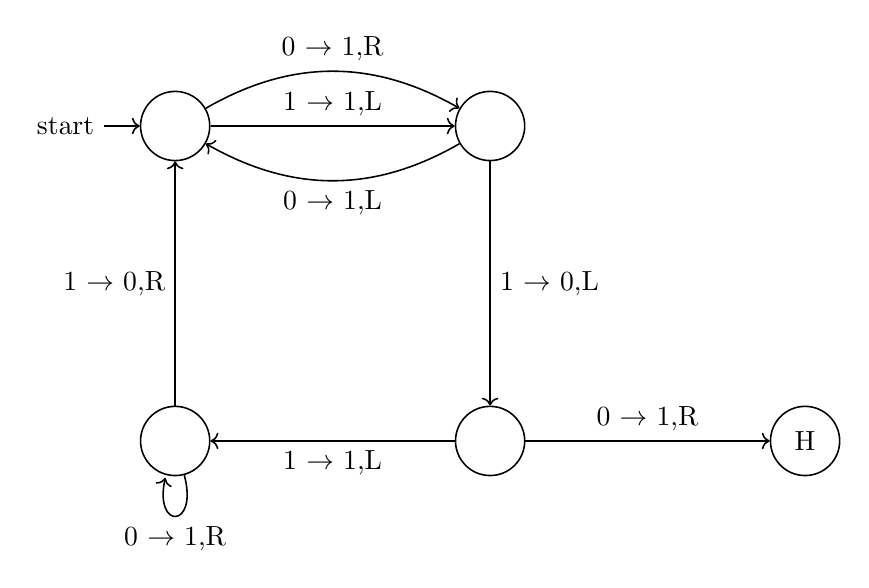
\begin{tikzpicture}[->,auto,node distance=4cm,line width=0.2mm]
  \node[initial,state] 		(A)            			{};
  \node[state] 			(B) [below of=A]   	{};
  \node[state] 			(C) [right of=A]    		{};
  \node[state] 			(D) [below of=C] 		{};
  \node[state]         		(E) [right of=D] 		{H};

  \path 	(A) edge node 				{1 $\rightarrow$ 1,L} 		(C)
		(A) edge [bend left] node 		{0 $\rightarrow$ 1,R} 		(C)
		(C) edge [bend left] node 		{0 $\rightarrow$ 1,L} 		(A)
		(B) edge node 				{1 $\rightarrow$ 0,R} 		(A)
		(B) edge [loop below] node 	{0 $\rightarrow$ 1,R} 		(B)
		(D) edge node 				{1 $\rightarrow$ 1,L} 		(B)
		(C) edge node 				{1 $\rightarrow$ 0,L} 		(D)
		(D) edge node		 		{0 $\rightarrow$ 1,R} 		(E);
\end{tikzpicture}
\end{center}

\begin{Verbatim}[fontsize=\small, frame=single]
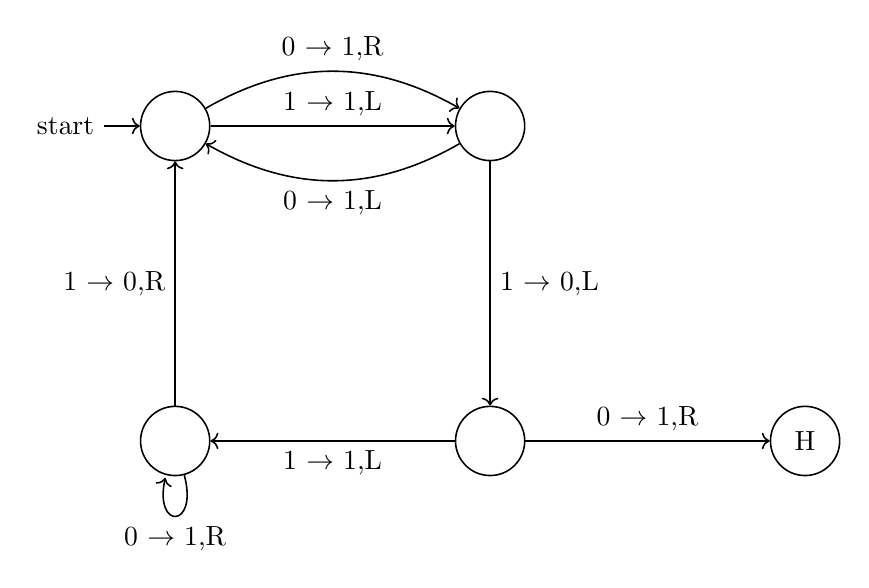
\begin{tikzpicture}[->,auto,node distance=4cm,line width=0.2mm]
  \node[initial,state] (A)              {};
  \node[state] 	(B) [below of=A] {};
  \node[state] 	(C) [right of=A] {};
  \node[state] 	(D) [below of=C] {};
  \node[state]         (E) [right of=D] {H};

  \path (A) edge node   	   {1 $\rightarrow$ 1,L}  (C)
	(A) edge [bend left] node  {0 $\rightarrow$ 1,R}  (C)
	(C) edge [bend left] node  {0 $\rightarrow$ 1,L}  (A)
	(B) edge node 	     {1 $\rightarrow$ 0,R} (A)
	(B) edge [loop below] node {0 $\rightarrow$ 1,R}  (B)
	(D) edge node 	     {1 $\rightarrow$ 1,L}  (B)
	(C) edge node 	     {1 $\rightarrow$ 0,L}  (D)
	(D) edge node	      {0 $\rightarrow$ 1,R}  (E);
\end{tikzpicture}
\end{Verbatim}

\newpage

%%% LOGISKE PORTER %%%
\section{Logiske porter}
Noe som er kjekt å vite om er også logiske porter i Circuitikz. Dette får du ved å inkludere pakken:
\begin{Verbatim}[fontsize=\small]
\usepackage{circuitikz}
\end{Verbatim}

Siden dette \textit{ikke} er TikZ jobber vi ikke i miljøet \texttt{tikzpicture}, men i miljøet \texttt{circuitikz}.

\begin{Verbatim}[fontsize=\small, frame=single]
\begin{circuitikz} \draw
    <kode her>
\end{circuitikz}
\end{Verbatim}

\subsection{Eksempel på en liten krets}

\begin{center}
\begin{circuitikz} \draw
(-3,0.3) node[not port] (not) {}
(0,0) node[and port] (and) {}
(2,1) node[or port] (or) {}
(not.out) -- (and.in 1)
(and.out) -- (or.in 2);
\end{circuitikz}
\end{center}

\begin{Verbatim}[fontsize=\small, frame=single]
\begin{circuitikz} \draw
    (-3,0.3) node[not port] (not) {}
    (0,0)    node[and port] (and) {}
    (2,1)    node[or port]  (or)  {}

    (not.out) -- (and.in 1)
    (and.out) -- (or.in 2);
\end{circuitikz}
\end{Verbatim}

Det fungerer på samme måte som når vi tegner noder i TikZ. Vi starter med koordinatene, så definerer vi hva slags node (port) vi vil ha, og til slutt en evt. merkelapp.

\begin{Verbatim}[fontsize=\small]
(x,y) node [what kind of port] (name of port) {label}
\end{Verbatim}

Portens navn er valgfritt, og brukes kun i din egen kode. 

\newpage

\subsection{Oversikt over forskjellige porter i Circuitikz}
\begin{figure}[h!]
\centering
\begin{tabular}{ll}
\texttt{[and port]} & \begin{circuitikz} \draw (0,0) node[and port] (myand1) {}; \end{circuitikz}\\
\texttt{[or port]} & \begin{circuitikz} \draw (0,0) node[or port] (myand1) {}; \end{circuitikz}\\
\texttt{[not port]} & \begin{circuitikz} \draw (0,0) node[not port] (myand1) {}; \end{circuitikz}\\
\texttt{[nand port]} & \begin{circuitikz} \draw (0,0) node[nand port] (myand1) {}; \end{circuitikz}\\
\texttt{[nor port]} & \begin{circuitikz} \draw (0,0) node[nor port] (myand1) {}; \end{circuitikz}\\
\texttt{[xor port]} & \begin{circuitikz} \draw (0,0) node[xnor port] (myand1) {}; \end{circuitikz}\\
\end{tabular}
\caption{Forskjellige porter i Circuitikz}
\end{figure}

\newpage

\section{Resursser}
\subsection*{Gøyale eksempler}
\begin{itemize}
	\item
	\href{http://www.texample.net/tikz/examples/enderman/}{Enderman}

	\item
	\href{http://www.texample.net/tikz/examples/dartboard/}{Dartboard}

	\item
	\href{http://www.texample.net/tikz/examples/india-map/}{India map}
\end{itemize}

\subsection*{Lære mer?}
\begin{itemize}
	\item
	\href{https://www.sharelatex.com/blog/2013/09/02/tikz-series-pt4.html}{Introduksjon til Circuitikz}

	\item
	\href{https://www.sharelatex.com/blog/2013/09/04/tikz-series-pt5.html}{Tankekart med TikZ}

	\item
	\href{https://www.sharelatex.com/blog/2013/08/28/tikz-series-pt2.html}{Generere TikZ-kode fra GeoGebra}
\end{itemize}

\end{document}